\section{系统设计}
\label{sec:method}

\subsection{时序子帧分解}

给定归一化原始帧 $\mathbf{I}\in[0,1]^{H\times W\times C}$，我们生成二值掩模 $\mathbf{M}_1,\ldots,\mathbf{M}_n$，使其满足 $\sum_{k=1}^{n}\mathbf{M}_k=\mathbf{1}$，并令 $\mathbf{I}_k=\mathbf{I}\odot\mathbf{M}_k$。由此得到：
\begin{itemize}
\item \textbf{数字域完备性}：$\sum_{k=1}^{n}\mathbf{I}_k = \mathbf{I}$；
\item \textbf{互斥性}：每个像素恰好在 $n$ 个时隙中的一个时隙内被点亮。
\end{itemize}
这里必须区分“求和”与“时域平均”。对于时隙持续时间和峰值亮度均相同的理想线性显示器，一个周期内的平均辐亮度是 $\mathbf{I}/n$，而不是 $\mathbf{I}$。数字域完备性表示可以对各子帧重新求和；它并不意味着真实显示器的亮度得到无损保留。

这一区别同时构成实验局限。物理拍摄研究未纳入亮度匹配的静态调暗对照、与增强档相匹配的无噪声版本，也未进行面板时序的光度测量。因而，观察到的档位级下降不能仅归因于时序稀疏性；占空比亮度、静态条纹/字形叠加、面板响应、相机曝光以及图像信号处理器（ISP）处理仍相互混杂。

像素分配由基于 ChaCha20~\cite{b_chacha2008} 的密码学安全伪随机数生成器（CSPRNG）产生。拒绝采样将字节流映射为无偏的时隙索引；另行采用 Fisher--Yates 洗牌~\cite{b_knuth1997} 随机化子帧播放顺序。卡方时隙计数检验（$\alpha=0.01$，$\mathrm{df}=n{-}1=3$）仅用作实现的健全性检查，最多重新采样 5 次，并不构成密码学强度的证据。随机化可减少固定图案与跨周期相关性，但无法阻止对已配准完整周期的线性重建。图~\ref{fig:pipeline} 展示了完整管线。

\begin{figure*}[!t]
\centering

\includegraphics[width=\textwidth,viewport=0 0 515.52 206.16,clip]{figures/visio/figure2_method_pipeline/final/figure2_method_pipeline.pdf}
\caption{从源内容到受保护显示的时序像素掩蔽系统管线。输入帧被分解为由 CSPRNG 分配的互补像素掩模；随后在高刷新率播放前，插入可选的面向 OCR 的互补噪声、与档位相关的条纹/字形叠加，以及可选的部分反色帧。人类观察者预期可将多个时隙整合为可读视图，而短曝光相机可能仅捕获一个稀疏子帧。长曝光和视频时域平均能够累积多个时隙，因此本文将其作为边界攻击单独评估，而非假定其不存在。}
\label{fig:pipeline}
\end{figure*}

\subsection{互补对抗噪声}

我们在子帧上叠加对抗噪声 $\mathbf{N}_1, \ldots, \mathbf{N}_n$，使其满足：
\begin{equation}
\sum_{k=1}^{n}\mathbf{N}_k = \mathbf{0}
\label{eq:noise_complement}
\end{equation}
式~(\ref{eq:noise_complement}) 仅在求和、裁剪和显示传递函数之前的理想线性域中严格成立。已有研究表明，较小的文本图像扰动即可显著误导 OCR 系统~\cite{b_song2018}，这为面向 OCR 的噪声设计提供了依据。噪声方向由快速梯度符号法（FGSM）式~\cite{b_goodfellow2015} 代理梯度生成，幅度上界为 $\varepsilon=8/255$，随后在时域中进行互补分解。由于显示器无法发出负辐亮度，实现中采用了基底电平和数值裁剪。因此，在伽马校正、量化、裁剪和相机成像之后，噪声不保证能在物理上相互抵消。

\textbf{组件作用}：随机点阵掩模是主要时序机制。互补噪声是理想域中的可选组件；条纹/字形叠加与部分反色是下述增强档使用的非线性附加项。本文保留归档复合档位的定义，不在事后移除其中的组件。这样可以保持与已拍摄数据的对应关系，但不能证明各组件的收益或最优性。在物理拍摄结果中，噪声效果并不单调，且未拍摄与增强档相匹配的无噪声版本。因此，我们解释的是完整档位，而不建议将互补噪声作为默认组件。

\subsection{亮度补偿}

每个像素在一个 $n$ 时隙周期内仅被点亮一次。如果显示器能够在像素激活的时隙内将线性光域的光输出提高到 $n$ 倍，则周期平均亮度将接近原始亮度。当前概念验证（PoC）既未实现逐时隙动态背光协同，也未进行光度验证。所有亮度对齐、CIEDE2000 $\Delta E_{00}$~\cite{b_ciede2000} 和 SSIM~\cite{b_wang2004} 结果均来自数字积分/归一化模型，仅用于跨配置比较，不构成真实面板在光学上等效或用户感到舒适的证据。

\subsection{时序与带宽}

对于仅包含 $n$ 个互补子帧的基础周期，若以 60\,Hz 作为最低周期率，则要求 $f_r\geq60n$；当 $n=4$ 时，对应 240\,Hz。如果周期还包含一个反色帧，则要求变为 $f_r\geq60(n+1)$，在 240\,Hz 下实际周期率将降至仅 48\,Hz。因此，240\,Hz 满足基础四子帧配置，却不能满足含反色帧配置的 60\,Hz 周期目标。人类闪烁感知还受亮度、对比度、视网膜偏心度、空间内容和眼动影响~\cite{b_cai2024,b_davis2015}；仅凭标称周期率无法预测舒适度。

观察者能否将互补子帧整合成感知完整的图像，取决于时间对比敏感函数（TCSF）。临界闪烁融合频率（CFF）并非普适的截止值：Davis 等人~\cite{b_davis2015} 发现，对于均匀调制，人眼在常规频率附近仍具有敏感性；而在存在高频空间边缘时，超过 500\,Hz 仍可能被观察到。因此，含反色配置的 48\,Hz 完整周期率可能令部分观察者察觉闪烁，基础配置的 60\,Hz 也不能被假定为无闪烁。只有计划中的用户研究才能确定这两种配置是否支持舒适的时序整合。

\subsection{探索性高抑制档}
\label{sec:hardened}

基础线性时序掩模在完整周期时域平均下会发生泄漏（见 \S\ref{sec:security_frontier}）。为应对此问题，我们引入非线性增强档。除非另有说明，本小节各档位均采用 $n=4$ 的基础时序掩蔽，并启用互补对抗噪声。表~\ref{tab:profile_composition} 汇总全部档位配置；表~\ref{tab:real_ocr_full_pool} 中的“掩蔽加噪声”行是不含条纹/字形抗 OCR 叠加的基础条件。

\begin{table*}[!t]
\caption{档位组成汇总（所有档位均取 $n=4$）}
\label{tab:profile_composition}
\centering
\footnotesize
\setlength{\tabcolsep}{3.2pt}
\begin{tabular}{lccccccc}
\toprule
档位 & 掩模 & 噪声 & 单元（px） & 条纹宽度（px） & 条纹 $\alpha_s$ & 字形 $\alpha_g$ & 反色 $\alpha$ \\
\midrule
仅掩蔽 & \checkmark & -- & 1 & -- & -- & -- & -- \\
掩蔽加噪声 & \checkmark & \checkmark & 1 & -- & -- & -- & -- \\
Strong & \checkmark & \checkmark & 1 & 10 & 0.10 & 0.12 & -- \\
可读性优先档 & \checkmark & \checkmark & 1 & 10 & 0.10 & 0.12 & 0.2 \\
高抑制档 & \checkmark & \checkmark & 2 & 6 & 0.42 & 0.55 & 0.2 \\
\bottomrule
\end{tabular}
\end{table*}

\begin{itemize}
\item \textbf{Strong（抗 OCR）档}：基础掩模加噪声，掩模单元大小为 1~像素，条纹宽度为 10~像素，条纹幅度 $\alpha_s=0.10$，字形幅度 $\alpha_g=0.12$，不含反色帧。

\item \textbf{可读性优先档}：在 Strong 档基础上加入一个 $\alpha=0.2$ 的反色帧，本文将其指定为面向可用性的复合配置。归档结果表与拍摄元数据使用标签“deployed”，但这一旧标识既不表示部署建议，也不是经过实证优化的证据。

\item \textbf{高抑制档}：一种探索性的安全导向压力测试档，采用基础掩模加噪声，将掩模单元大小增至 2~像素，条纹宽度设为 6~像素，条纹和字形幅度分别为 0.42 和 0.55，并加入一个 $\alpha=0.2$ 的反色帧。
\end{itemize}

非线性档偏离严格完备性（$\sum\mathbf{I}_k \neq \mathbf{I}$），会产生可见条纹与颗粒。这一取舍与 Kaleido 类时序重编码相反：后者依赖周期内在感知上完整的混合来维持观看体验，这意味着完整周期积分必然重建出原始画面的近似结果，与其防盗录目标相符。而在本文处理的静态内容拍摄威胁中，完备性恰恰是积分攻击的切入点；高抑制档主动将破坏严格完备性作为设计取舍，以可见条纹和颗粒为代价，换取完整周期积分下较低的恢复率。其安全收益和未经测量的可读性代价必须分别报告，也不应将其视为经过用户验证的候选部署方案。

本文采用“高抑制”这一论文表述，因为它只描述该档位在表~\ref{tab:profile_composition} 中的相对位置，并不暗示已经达到某项抗拍摄目标，也不暗示用户能够容忍该档位。为保证可复现性，归档标识仍为 \texttt{capture\_hardened}（旧标签为 \texttt{vlm}）；\S\ref{sec:real_capture} 报告其未达到目标以及残余泄漏。

\subsection{部分反色帧}

当曝光窗口覆盖一个完整显示周期时，即构成长曝光攻击（$n=4$、240\,Hz 时，基础周期约为 16.7\,ms；加入反色帧后，$n+1$ 时隙周期约为 20.8\,ms）。归档中的长曝光标签 31.25 和 125\,ms 是根据 UVC 控制量推导的标称值，而非光度测量值。在归一化域 $\mathbf{I}\in[0,1]$ 中，实现会在每个 $n$ 子帧周期后插入一个\textbf{部分反色帧} $\alpha(\mathbf{1}-\mathbf{I})$。其等价的 8 位表达式为 $\alpha(255-\mathbf{I}_{8})$。增大 $\alpha$ 会同时改变积分信号，以及数字重建结果的亮度和对比度。

真机拍摄的反色强度消融（表~\ref{tab:inversion_ablation}；管线见 \S\ref{sec:real_capture}）显示，$\alpha=0$ 时恢复率为 68.6\%，$\alpha=0.2$ 时为 67.0\%。在 $\alpha\in[0,0.5]$ 范围内，各点估计值介于 61.7\% 和 72.0\% 之间；拍摄样本重采样区间仅用于描述，区间重叠也不是等效性检验。该消融固定 Strong 叠加层，并使用由五项账号/代码/CET6 内容组成的子集。其 $\alpha=0.2$ 数值（$N=135$）并非对可读性优先行的重复估计。接近全反色（$\alpha=1.0$）时，观察到的恢复率降至 18.1\%，但数字积分视图也严重退化。在 150 帧时域均值下，弱反色设置仍保留 64--73\% 的恢复率。可读性优先档选择 $\alpha=0.2$ 是一种模型化设计决策，而非经过验证的最优值。

\begin{table}[!t]
\caption{固定 Strong 叠加层（$\alpha_s=0.10$，$\alpha_g=0.12$）上的反色帧强度 $\alpha$ 消融：真机拍摄引擎最优字符恢复率（均值与 95\% 拍摄样本重采样区间，汇总 9 个几何条件下的五项账号/代码/CET6 内容；长曝光每个设置 $N=135$，视频时域平均每个设置 $N=45$）。该五项子集不同于表~\ref{tab:real_ocr_full_pool} 中可读性优先行使用的 12 项内容。}
\label{tab:inversion_ablation}
\centering
\footnotesize
\begin{tabular}{lcc}
\toprule
$\alpha$ & 长曝光字符（\%） & 视频均值字符（\%） \\
\midrule
0.0 & 68.6~[63.1, 73.9] & 72.7~[63.3, 81.1] \\
0.2 & 67.0~[61.3, 72.7] & 69.8~[59.9, 78.7] \\
0.3 & 72.0~[66.2, 76.9] & 64.3~[54.0, 73.6] \\
0.5 & 61.7~[55.6, 67.7] & 66.4~[56.5, 75.2] \\
1.0 & 18.1~[14.0, 22.0] & 28.4~[20.5, 36.9] \\
\bottomrule
\end{tabular}
\end{table}

因此，每个显示周期包含 $n+1$ 个时隙。当 $n=4$ 且刷新率为 240\,Hz 时，周期率为 48\,Hz，低于 60\,Hz 的设计目标，并可能产生可感知闪烁；不存在适用于所有观看条件的固定“无闪烁阈值”。

\subsection{实现范围}

当前 PoC 工作在应用/算法层，使用 Python 和图形处理器（GPU）渲染来生成显示序列。它不包含操作系统（OS）驱动级注入（DXGI / KMS-DRM / CoreDisplay），也不包含逐时隙动态背光控制。本文验证的是显示序列及其拍摄结果，并不声称已实现生产级系统集成。


%% ============================================================
%% V. 实验评估
%% ============================================================
\section{实验评估}
\label{sec:evaluation}

\subsection{实验设置}
\label{sec:setup}

\textbf{硬件平台}：大多数实验使用一台配备 Intel Core i7-8700K（3.70\,GHz）、32\,GB RAM 和 NVIDIA TITAN Xp（12\,GB VRAM）的桌面工作站。归档的 d0.5/$0^{\circ}$ 运行是在另一台采集机器上使用 $2560\times1600$ 播放画布完成的，但该机器的硬件规格未被保留；其余运行均使用 $1920\times1080$。显示器为 AOC 24G51Z，以标称 240\,Hz 驱动。标称 240-Hz 下，每个时隙持续 4.17\,ms；基础周期和加入反色帧后的周期率分别为 60 和 48\,Hz。面板转换行为未被测量，也不能根据刷新率规格推断。

\textbf{拍摄设备}：所有物理拍摄均使用一台 eMeet SmartCam S600 USB 网络摄像头及其标准 UVC 驱动。相机帧在识别前经过透视校正和内容裁剪。逐次拍摄元数据保存了由 DirectShow/UVC log$_2$ 控制量推导的曝光标签：$-11$ 和 $-8$ 分别标称映射为 0.49 和 3.91\,ms，$-5$ 和 $-3$ 分别映射为 31.25 和 125\,ms。八个几何条件使用共同的 $-8/-5$ 设置；d0.5/$15^{\circ}$ 使用 $-11/-3$。这些数值是推导得到的控制标签，并非实测快门时间。采集代码尝试采用手动曝光，但归档元数据未保存经过语义解码的自动曝光状态。增益、自动白平衡和对焦状态也未被保留。整个采集过程中，显示器亮度设置与采集相位保持固定，但未测量显示器的物理亮度。视频以标称 60\,fps 拍摄。主要 OCR 输入为经过几何校正的内容裁剪区域。

相机与显示器的距离分别为 0.5\,m、1\,m 和 1.5\,m，并在每个距离下分别旋转至 $0^{\circ}$、$15^{\circ}$ 和 $30^{\circ}$。环境照度未被记录。厂商标明该设备采用 8 百万像素 4K 传感器，并支持 1080p/60\,fps 输出~\cite{b_emeet_s600}，但没有说明传感器型号。滚动快门读出、面板输出和应用层时隙时序均未经过光度表征。行混合与面板转换可能解释仿真到真机之间的差距，但现有数据无法识别各自的贡献。结果仅适用于这一 UVC 链路。

\textbf{测试内容}：每个位置均使用 12 个固定内容项：两个账号字符串、两个代码片段、两个数字字符串、一个英文句子、两个混合语言片段、两个英文段落，以及一份 CET6（大学英语六级考试，College English Test Band~6）文档。CET6 页面含有中文文本，两个混合语言内容项也含有中文字符；因此，该语料并非全英文或全 ASCII。11 个合成内容项旨在覆盖上述内容形式，但从 120 个样本的仿真语料中选择这些内容项的过程并未预注册。三次重复使每个档位--攻击--位置单元包含 36 次拍摄；计入已披露的重复采集之前，9 个位置合计为 324 次。检测与跟踪使用不同的子集，仅作为补充诊断。

\textbf{评估指标}：OCR 字符恢复率定义为 $\max(0,1-\mathrm{CER})$，其中 CER 为字符错误率。完全匹配率在移除空白后，以不区分大小写的全文比较计算。显式字段恢复使用评分前固定的 18 个字段，覆盖 9 个含字段内容项。仅当某字段完整的 Unicode 归一化形式出现在该次拍摄至少一个引擎的输出中时，才将其计为已恢复；比较时忽略大小写、空白和标点。本文分别报告字段级微平均恢复率和样本级宏平均恢复率。泄漏率是字符恢复率 $\geq20\%$ 的样本比例，仅作为描述性阈值。在匹配的共同设置单元上，可读性优先档字符恢复率的 P50、P75、P90、P95 和 P99 分别为 10.1\%、22.0\%、45.6\%、63.6\% 和 95.0\%。高抑制档对应值分别为 3.4\%、9.2\%、15.2\%、19.1\% 和 22.6\%。

\textbf{OCR 聚合与不确定性}：对于每次拍摄，字符指标与全文指标分别在三个引擎中取最大值。显式字段采用三个引擎所恢复字段的并集。在匹配前，先对档位、内容、位置和重复编号相同的重复拍摄取平均。主要比较使用三个档位中都存在的键。配对对比将 12 个内容项作为聚类进行重采样，共 2,000 次，随机种子为 20260612。这些内容项聚类区间将所测几何条件视为固定，不能估计新设备上的不确定性。表~\ref{tab:real_ocr_full_pool} 则给出不平衡归档的拍摄样本重采样汇总；这些区间用于描述，而非总体置信区间。在所有几何条件上，未保护条件的恢复率比可读性优先档高 78.0 个百分点（[75.5, 80.3]），比高抑制档高 89.1 个百分点（[85.0, 92.4]）。仅掩蔽档比可读性优先档高 3.0 个百分点（[-0.5, 6.5]），因此归档数据不能证明每个组件都具有独立收益。

\textbf{共同设置分析}：d0.5/$15^{\circ}$ 位置采用了不同的标称 UVC 设置，并产生了明显欠曝的受保护帧。其余 8 个几何条件构成主要固定设置结果（表~\ref{tab:real_ocr_common}）。经过重复采集平均和三个档位匹配后，每个档位均有 $N=288$ 个单元。未保护、可读性优先和高抑制档的平均恢复率分别为 94.5\%、17.8\% 和 5.6\%。配对对比分别为 76.7 个百分点（[74.3, 79.2]）和 88.9 个百分点（[85.5, 91.9]）。可读性优先档在不平衡拍摄图像集合中的平均值为 16.7\%，共 408 张图像，仅作为敏感性汇总报告。排除不可比较的几何条件后，可读性优先档的 150 帧视频均值恢复率由 71.1\% 升至 79.7\%，高抑制档则由 47.9\% 升至 53.9\%。

\textbf{其他稳健性检查}：对五个重复内容项进行留一轮分析，可读性优先档的短曝光恢复率在第 1 轮为 16.6\%，在第 2 轮为 15.8\%，档位级解释未发生变化。检测与跟踪差异尚未进行显著性检验，仅在补充材料中作描述性报告。

\textbf{固定预处理压力测试}：我们在全部 984 张选定的主要样本池图像上评估了 Tesseract、EasyOCR 和 Surya。固定输入网格包含原始输入、gamma 0.5、亮度对比度受限自适应直方图均衡化（CLAHE；第 1--99 百分位拉伸，裁剪限值 4.0，$8\times8$ 分块）、非锐化掩蔽（$\sigma=1.0$，权重 1.7/$-0.7$）、高斯自适应阈值化（块大小 31，常数 5），以及 2$\times$ 双三次上采样。所有参数均在评分前固定。对于每项指标和每次拍摄，攻击者保留最佳引擎--输入组合；随后先对重复拍摄取平均，再执行与主要分析相同的三个档位匹配。完整矩阵包含 17,712 个单元（984 张图像 $\times$ 6 种输入形式 $\times$ 3 个引擎），且未出现 OCR 错误。非原始输入的 Tesseract 单元通过 \texttt{pytesseract 0.3.13} 调用 Tesseract 5.4.1；EasyOCR 1.7.2 和 Surya 0.14.7 的变换输入单元在上述工作站上使用 CUDA。原始输入单元从主要归档导入，其中未保存 Windows 版 Tesseract/EasyOCR 的确切构建版本。该固定网格最优选择（oracle）在声明的网格内对攻击者有利，但它不是无约束自适应搜索、学习式增强攻击或商业 OCR 上界。

数字重建代理指标：$\Delta E_{00}$ 是原始图像与完整周期数字重建图像之间的平均 CIEDE2000 色差；SSIM~\cite{b_wang2004} 是二者的平均结构相似度。两项指标均在数字管线中计算，仅用于本文内部的档位比较。两者均不能衡量真实面板的光学输出、时序舒适度或人类可读性。

% ----------------------------------------------------------
\subsection{真机拍摄 OCR 实验}
\label{sec:real_capture}

物理拍摄归档共包含 10,575 张图像（每个位置 1,175 张），全部来自 S600 网络摄像头。该总数混合了消融、参数扫描与主要攻击条件。可读性优先档对 12 个内容项中的 5 项包含第二轮采集，因此全位置短曝光/视频图像数为 459/153，而不是 324/108。匹配对比前先对重复键取平均。没有采集第二批长曝光数据。Surya~\cite{b_surya2024}、EasyOCR~\cite{b_easyocr2020} 和 Tesseract~\cite{b_smith2007} 共生成 31,725 条引擎级记录。Surya 重跑固定使用 \texttt{surya-ocr 0.14.7}；结果归档未嵌入 Windows 版 Tesseract 和 EasyOCR 的确切构建版本，这仍是一项可复现性局限。每个几何条件使用归档的四点单应变换和输出画布，随后应用已记录的内容裁剪；主要 OCR 管线不包含其他自适应增强。各档位按照 original、mask-only、mask+noise、Strong、可读性优先和高抑制的固定顺序采集，没有随机化。时间漂移或批次漂移可能混杂档位比较。主要比较采用 8 个共同设置几何条件，而表~\ref{tab:real_ocr_full_pool} 保留全部 9 个条件作为敏感性证据。图~\ref{fig:montage} 展示了 1.0\,m/$0^{\circ}$ 下的数字重建结果和匹配的共同设置拍摄结果。

\begin{table*}[!t]
\caption{共同标称 3.91-ms UVC 设置下主要匹配短曝光 OCR 比较。匹配前先对重复拍摄取平均；每个档位的 $N=288$ 由 12 个内容项 $\times$ 8 个几何条件 $\times$ 3 次重复组成。排除不可比较的 d0.5/$15^{\circ}$ 运行。}
\label{tab:real_ocr_common}
\centering
\footnotesize
\setlength{\tabcolsep}{4.6pt}
\begin{tabular}{lcccl}
\toprule
档位 & $N$ & 平均字符恢复率 & 未保护 $-$ 该档位 & 解释 \\
\midrule
原始（未保护） & 288 & 94.5\% & -- & 共同设置基线 \\
可读性优先档 & 288 & 17.8\% & 76.7\,个百分点 [74.3, 79.2] & 传统 OCR 恢复下降，但上尾仍有失效 \\
高抑制档 & 288 & 5.6\% & 88.9\,个百分点 [85.5, 91.9] & 探索性压力测试档；未达到严格的 $<5\%$ 目标 \\
\bottomrule
\end{tabular}
\end{table*}

\begin{table}[!t]
\caption{主要匹配短曝光样本池中的显式敏感字段完全恢复率。18 个字段在评分前固定；每个档位的 288 个单元中，有 216 个至少包含一个字段。}
\label{tab:explicit_fields}
\centering
\footnotesize
\begin{tabular}{lcc}
\toprule
档位 & 字段微平均（432 次机会） & 样本宏平均 \\
\midrule
原始（未保护） & 91.4\% & 86.8\% \\
可读性优先档 & 17.7\% & 17.5\% \\
高抑制档 & 1.2\% & 1.1\% \\
\bottomrule
\end{tabular}
\end{table}

\begin{table*}[!t]
\caption{单一 UVC 真机拍摄 OCR 敏感性样本池（引擎最优；$N$ 为每行拍摄数；包含全部 9 个几何条件）。方括号内为 95\% 拍摄样本重采样汇总，而非总体置信区间。视频行对 150 帧取平均。主要匹配估计见表~\ref{tab:real_ocr_common}。}
\label{tab:real_ocr_full_pool}
\centering
\footnotesize
\begin{tabular}{lllccc}
\toprule
档位 & 攻击模式 & $N$ & 字符恢复率 [95\% 汇总] & 完全匹配率 & 泄漏率 \\
\midrule
\multirow{3}{*}{原始（未保护）}
 & 短曝光 & 324 & 94.1 [93.1, 95.0]\% & 65.7\% & 99.4\% \\
 & 视频（150 帧均值） & 108 & 79.9 [73.5, 86.0]\% & 61.1\% & 86.1\% \\
 & 长曝光 & 324 & 47.3 [42.8, 51.9]\% & 18.8\% & 58.6\% \\
\midrule
\multirow{3}{*}{仅掩蔽}
 & 短曝光 & 324 & 19.2 [17.0, 21.4]\% & 0.3\% & 30.6\% \\
 & 视频（150 帧均值） & 108 & 79.0 [73.0, 84.9]\% & 48.1\% & 88.0\% \\
 & 长曝光 & 324 & 67.2 [63.0, 71.5]\% & 35.5\% & 75.0\% \\
\midrule
\multirow{3}{*}{掩蔽加噪声}
 & 短曝光 & 324 & 25.6 [22.5, 28.8]\% & 2.8\% & 36.1\% \\
 & 视频（150 帧均值） & 108 & 79.2 [73.3, 85.0]\% & 49.1\% & 88.9\% \\
 & 长曝光 & 324 & 68.0 [63.7, 72.4]\% & 39.8\% & 76.2\% \\
\midrule
\multirow{3}{*}{Strong（抗 OCR）}
 & 短曝光 & 324 & 20.7 [18.2, 23.3]\% & 0.6\% & 32.4\% \\
 & 视频（150 帧均值） & 108 & 78.6 [72.5, 84.5]\% & 50.9\% & 88.9\% \\
 & 长曝光 & 324 & 61.6 [57.1, 66.1]\% & 39.8\% & 71.3\% \\
\midrule
\multirow{3}{*}{可读性优先档}
 & 短曝光 & 459 & 15.1 [13.3, 17.1]\% & 0.4\% & 20.5\% \\
 & 视频（150 帧均值） & 153 & 71.1 [65.7, 76.2]\% & 42.5\% & 85.0\% \\
 & 长曝光 & 324 & 60.9 [56.6, 65.6]\% & 36.4\% & 69.1\% \\
\midrule
\multirow{3}{*}{高抑制档}
 & 短曝光 & 324 & 5.0 [4.3, 5.8]\% & 0.0\% & 3.7\% \\
 & 视频（150 帧均值） & 108 & 47.9 [41.8, 54.0]\% & 5.6\% & 76.9\% \\
 & 长曝光 & 324 & 9.3 [7.9, 10.9]\% & 0.0\% & 14.2\% \\
\bottomrule
\end{tabular}
\end{table*}

\textbf{主要发现}：

\begin{enumerate}
\item \textbf{主要固定设置证据}：表~\ref{tab:real_ocr_common} 给出主要短曝光估计。每个档位均使用相同的 288 个匹配单元（12 个内容项 $\times$ 8 个几何条件 $\times$ 3 次重复），未保护、可读性优先和高抑制档的平均恢复率分别为 94.5\%、17.8\% 和 5.6\%。配对的内容项聚类对比分别为 76.7 个百分点（[74.3, 79.2]）和 88.9 个百分点（[85.5, 91.9]）。包含全部 9 个几何条件的拍摄图像池给出的数值为 94.1\%、15.1\% 和 5.0\%，但该样本池混合了不同曝光设置和重复采集。因此，得到支持的结果仅限于这一单相机、标称设置管线。

\item \textbf{固定预处理实质性削弱了原始输入结果}：在每个档位相同的 288 个匹配单元上，原始输入的三引擎最优选择给出 94.5\% 的未保护恢复率、17.8\% 的可读性优先档恢复率和 5.6\% 的高抑制档恢复率。允许五种固定变换后，这些数值分别升至 95.9\%、40.2\% 和 13.7\%（表~\ref{tab:preprocessing_grid}）。在这一更强的传统 OCR 条件下，未保护减可读性优先的配对差值为 55.7 个百分点（[50.3, 60.5]），未保护减高抑制的差值为 82.2 个百分点（[78.5, 85.2]）。包含 17,712 个单元的矩阵没有出现 OCR 错误。这些结果排除了“原始输入数值构成传统预处理攻击上界”的主张，但仍未评估无约束增强和商业 OCR。

\item \textbf{档位组件与目标边界}：在汇总归档中，仅掩蔽条件达到 19.2\%，掩蔽加噪声达到 25.6\%，Strong 达到 20.7\%。因此，归档不能证明噪声或弱叠加具有单调收益。可读性优先档是一项复合观察结果，而不是每个组件均有帮助的证据。在匹配样本池中，该档位仍有 17.7\% 的字段微平均完全恢复率（表~\ref{tab:explicit_fields}）和 95.0\% 的 P99 字符恢复率。高抑制档同样未达到其描述性的 $<5\%$ 目标；在共同标称设置下，其匹配平均值为 5.6\%。

\item \textbf{积分攻击仍是残余失效边界}（图~\ref{fig:bar_attack}）：在标称长曝光下，可读性优先档的字符恢复率为 60.9\%，完全匹配率为 36.4\%；在 150 帧均值下，二者分别为 71.1\% 和 42.5\%。排除 d0.5/$15^{\circ}$ 后，视频恢复率升至 79.7\%。弱反色（$\alpha=0.2$）并未产生显著的观测积分恢复下降。仅掩蔽档和 Strong 档在 150 帧均值下也较为接近（79.0\% 对 78.6\%）。这些比较仅用于描述，不能隔离组件因果效应。高抑制档的积分恢复率较低，但仍存在大量泄漏。

\item \textbf{长曝光反转是一项值得注意的负面结果}：未保护条件的长曝光字符恢复率基线仅为 47.3\%，低于可读性优先档的 60.9\%。在唯一采用 125\,ms 的位置（0.5\,m/$15^{\circ}$），未保护恢复率为 1.1\%，可读性优先档则为 46.3\%；全亮图像中观察到的裁剪现象支持以下解释：亮度降低减少了饱和，使信号移入传感器近似线性的响应区域。排除该位置后，31.25\,ms 异常仍随位置变化：在 0.5\,m 下，结果符合预期方向（未保护 78--82\% $>$ 可读性优先 25--55\%）；而在六个 1.0--1.5\,m 位置中，有五个位置的可读性优先档恢复率高出 1.9--59\,个百分点（其中四个超过 12\,个百分点）。由于缺少匹配的局部图像诊断，我们仅\emph{假设}残余条纹/字形边缘会与几何条件特定的过曝或对比度压缩相互作用；现有数据不能确立该机制。这一异常不削弱短曝光结论，因为可读性优先档在短曝光下始终更低；但它表明固定长曝光参数会产生非单调效应。主要有效性结论限于单帧短曝光；积分攻击作为安全边界报告。

\item \textbf{高抑制档：积分泄漏降低，但感知代价尚未解决}：这一探索性压力测试档在标称长曝光下得到 9.3\% 字符恢复率 [7.9, 10.9] / 0\% 完全匹配率，在 150 帧均值下得到 47.9\% 字符恢复率 [41.8, 54.0] / 5.6\% 完全匹配率 [1.9, 10.2]。方括号内为拍摄样本重采样汇总。汇总均值掩盖了较大的位置间差异，其中包括一个恢复率为 0\% 的欠曝会话。排除该会话后，视频恢复率升至 53.9\% [48.0, 59.9]，完全匹配率升至 6.3\%。任何部署评估都需要覆盖更广的几何条件、曝光、跨设备和用户可接受性证据。用户研究协议不包含该档位。

\item \textbf{几何趋势}：在 9~个条件（0.5--1.5\,m $\times$ 0--30$^{\circ}$）下，受保护短曝光的恢复率始终低于未保护值。由于实验设计不平衡，且未拟合几何因素的推断模型，我们不主张恢复率随距离或角度具有统计显著的单调鲁棒性。
\end{enumerate}

\begin{figure}[!t]
\centering
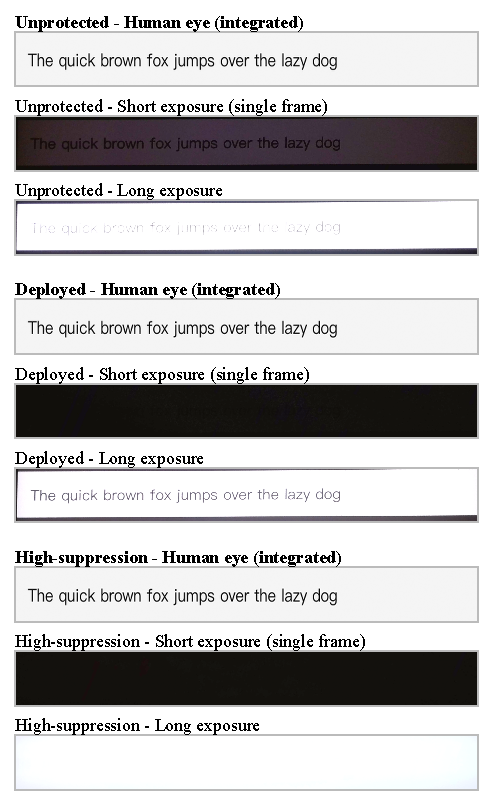
\includegraphics[width=\columnwidth]{figures/real_capture_montage.pdf}
\caption{1.0\,m、$0^{\circ}$ 条件下的真机拍摄蒙太奇。在纵向堆叠的每个档位组（未保护、可读性优先和高抑制）内，图像从上至下依次为数字积分重建、3.91\,ms 短曝光拍摄和 31.25\,ms 长曝光拍摄。相机图像以相同方式从归档原始相机 JPEG 中裁剪，未进行几何校正或亮度增益，因此与 OCR 评估使用的几何校正裁剪图不同。数字图像对每个档位均使用相同的 $1920\times1080$ 黑色播放画布和亮度对齐的完整周期积分；可读性优先和高抑制重建包含记录的 $\alpha=0.2$ 反色时隙。这些数字视图并非人类可读性或视觉舒适度的直接证据。}
\label{fig:montage}
\end{figure}

\begin{figure}[!t]
\centering

\includegraphics[width=\columnwidth]{figures/real_capture_bar.pdf}
\caption{三个代表性真机拍摄档位（未保护、可读性优先和高抑制）在短曝光、长曝光及 150 帧视频时域均值下的引擎最优 OCR 字符恢复率和完全匹配率，汇总全部 9 个所测距离--角度配置。柱越低，表示恢复出的文本越少。长曝光与视频柱揭示了积分边界：即使可读性优先档的短曝光柱较低，在积分攻击下仍保留大量可恢复内容。可读性优先档的样本数包含已披露的五项内容重复采集，因此与其他档位不同。}
\label{fig:bar_attack}
\end{figure}

\textbf{分引擎结果}：表~\ref{tab:real_ocr_engine} 按引擎拆分汇总的原始输入短曝光结果。不同引擎的未保护恢复率差异很大（Surya 37.1\%、EasyOCR 79.5\%、Tesseract 84.3\%）。Strong 条件下的恢复率范围为 2.1--16.3\%，可读性优先档为 3.2--11.7\%，高抑制档为 1.8--2.0\%。表~\ref{tab:preprocessing_grid} 和图~\ref{fig:real_engine_ocr} 则使用匹配的共同设置样本池，并表明每个引擎都至少受益于一种固定变换。对于可读性优先档，Tesseract 的恢复率由 3.2\% 升至 10.8\%，EasyOCR 由 14.2\% 升至 33.9\%，Surya 由 4.1\% 升至 20.2\%。对于高抑制档，相应变化分别为 2.0\% 至 8.2\%、2.3\% 至 6.5\%，以及 2.0\% 至 6.0\%。按指标选择的网格最优结果在这一有限的开源引擎与变换集合内对攻击者有利；本文未测试 Google Cloud Vision、Azure AI Vision 或百度 OCR 等商业 OCR 应用程序接口（API），这些服务可能取得更高恢复率，因此该结果并非现有 OCR 服务的上界。

\begin{table}[!t]
\caption{真机拍摄短曝光 OCR：分引擎结果（汇总 9 个几何条件）}
\label{tab:real_ocr_engine}
\centering
\footnotesize
\setlength{\tabcolsep}{5.5pt}
\begin{tabular}{llccc}
\toprule
档位 & 引擎 & 字符（\%） & 完全匹配（\%） & N \\
\midrule
\multirow{3}{*}{原始}
 & Surya & 37.1 & 22.8 & 324 \\
 & EasyOCR & 79.5 & 27.8 & 324 \\
 & Tesseract & 84.3 & 47.8 & 324 \\
\midrule
\multirow{3}{*}{仅掩蔽}
 & Surya & 4.2 & 0.3 & 324 \\
 & EasyOCR & 15.6 & 0.0 & 324 \\
 & Tesseract & 3.2 & 0.0 & 324 \\
\midrule
\multirow{3}{*}{掩蔽加噪声}
 & Surya & 11.0 & 2.8 & 324 \\
 & EasyOCR & 18.1 & 0.0 & 324 \\
 & Tesseract & 4.8 & 0.0 & 324 \\
\midrule
\multirow{3}{*}{Strong}
 & Surya & 6.1 & 0.6 & 324 \\
 & EasyOCR & 16.3 & 0.0 & 324 \\
 & Tesseract & 2.1 & 0.0 & 324 \\
\midrule
\multirow{3}{*}{可读性优先档}
 & Surya & 3.2 & 0.4 & 459 \\
 & EasyOCR & 11.7 & 0.0 & 459 \\
 & Tesseract & 3.3 & 0.0 & 459 \\
\midrule
\multirow{3}{*}{高抑制档}
 & Surya & 1.8 & 0.0 & 324 \\
 & EasyOCR & 2.0 & 0.0 & 324 \\
 & Tesseract & 1.9 & 0.0 & 324 \\
\bottomrule
\end{tabular}
\end{table}

\begin{table}[!t]
\caption{固定预处理网格下匹配共同设置的字符恢复率。每个单元格均为原始输入 $\rightarrow$ 逐次拍摄网格最优选择（\%）；重复采集平均和匹配后，每个档位 $N=288$。}
\label{tab:preprocessing_grid}
\centering
\footnotesize
\setlength{\tabcolsep}{4.2pt}
\begin{tabular}{lccc}
\toprule
引擎 & 原始 & 可读性优先 & 高抑制 \\
\midrule
Tesseract & 84.9 $\rightarrow$ 91.8 & 3.2 $\rightarrow$ 10.8 & 2.0 $\rightarrow$ 8.2 \\
EasyOCR & 85.1 $\rightarrow$ 88.4 & 14.2 $\rightarrow$ 33.9 & 2.3 $\rightarrow$ 6.5 \\
Surya & 30.6 $\rightarrow$ 49.3 & 4.1 $\rightarrow$ 20.2 & 2.0 $\rightarrow$ 6.0 \\
三者最优 & 94.5 $\rightarrow$ 95.9 & 17.8 $\rightarrow$ 40.2 & 5.6 $\rightarrow$ 13.7 \\
\bottomrule
\end{tabular}
\end{table}

\begin{figure}[!t]
\centering
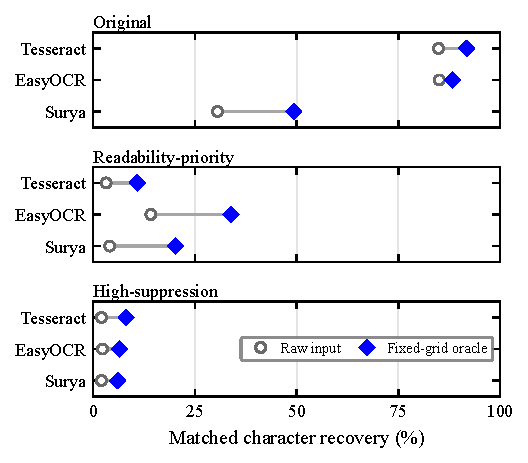
\includegraphics[width=\columnwidth]{figures/real_engine_ocr.pdf}
\caption{匹配共同设置样本池中，各 OCR 引擎的原始输入与固定网格最优字符恢复率对比（每个档位 $N=288$）。网格最优选择针对每次拍摄和每项指标，分别从原始输入加五种预先声明的变换中选取最佳结果。连线表示同一引擎内部的增幅，而非不确定性区间。确切数值见表~\ref{tab:preprocessing_grid}。}
\label{fig:real_engine_ocr}
\end{figure}
